\documentclass{beamer}
\usetheme{Warsaw}

\usepackage[utf8]{inputenc}
\usepackage{fancybox}
\usepackage{multimedia} 
\usepackage{subfig}
\usepackage{amsmath}
\usepackage{hyperref}
\usepackage{marvosym}

\usepackage[all]{xy}
\begin{document}


\title[Digitale Bildverarbeitung] % (optional, only for long titles)
{Digitale Bildverarbeitung
\\
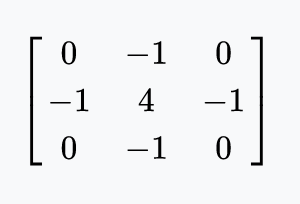
\includegraphics[scale=1.0]{img/cover}
}
\subtitle{}
\author[Dr. Johannes Riesterer] % (optional, for multiple authors)
{Dr.  rer. nat. Johannes Riesterer}

\date[KPT 2004] % (optional)
{}

\subject{Digitale Bildverarbeitung}

\frame{\titlepage}


\begin{frame}
    \frametitle{Lineare Filter}
\framesubtitle{}

\begin{block}{2 dimensionale Filtermasken}
Für ein diskretes Bild $U: Z^2 \to R$ und eine Filtermaske 
\begin{align*}
H := \begin{bmatrix} 
    H_{-r, -s} & \cdots  & H_{-r, s} \\
     \vdots & H_{0, 0} & \vdots						\\
	H_{r, -s} & \cdots & H_{r, s} 
\end{bmatrix}
\end{align*}
ist die Faltung in Anlehnung an den 1 dimensionalen Fall definiert durch
\begin{align*}
(U * H)_{i ,j}:=  \sum_{k = -r}^{r} \sum_{l = -s}^{s} H_{k,l} U_{i+k, j+l}
\end{align*}

\end{block}

 \end{frame}

\begin{frame}
    \frametitle{Lineare Filter}
\framesubtitle{}
\begin{block}{Fortsetzung am Bildrand}
\begin{figure}[htp]
      \centering
    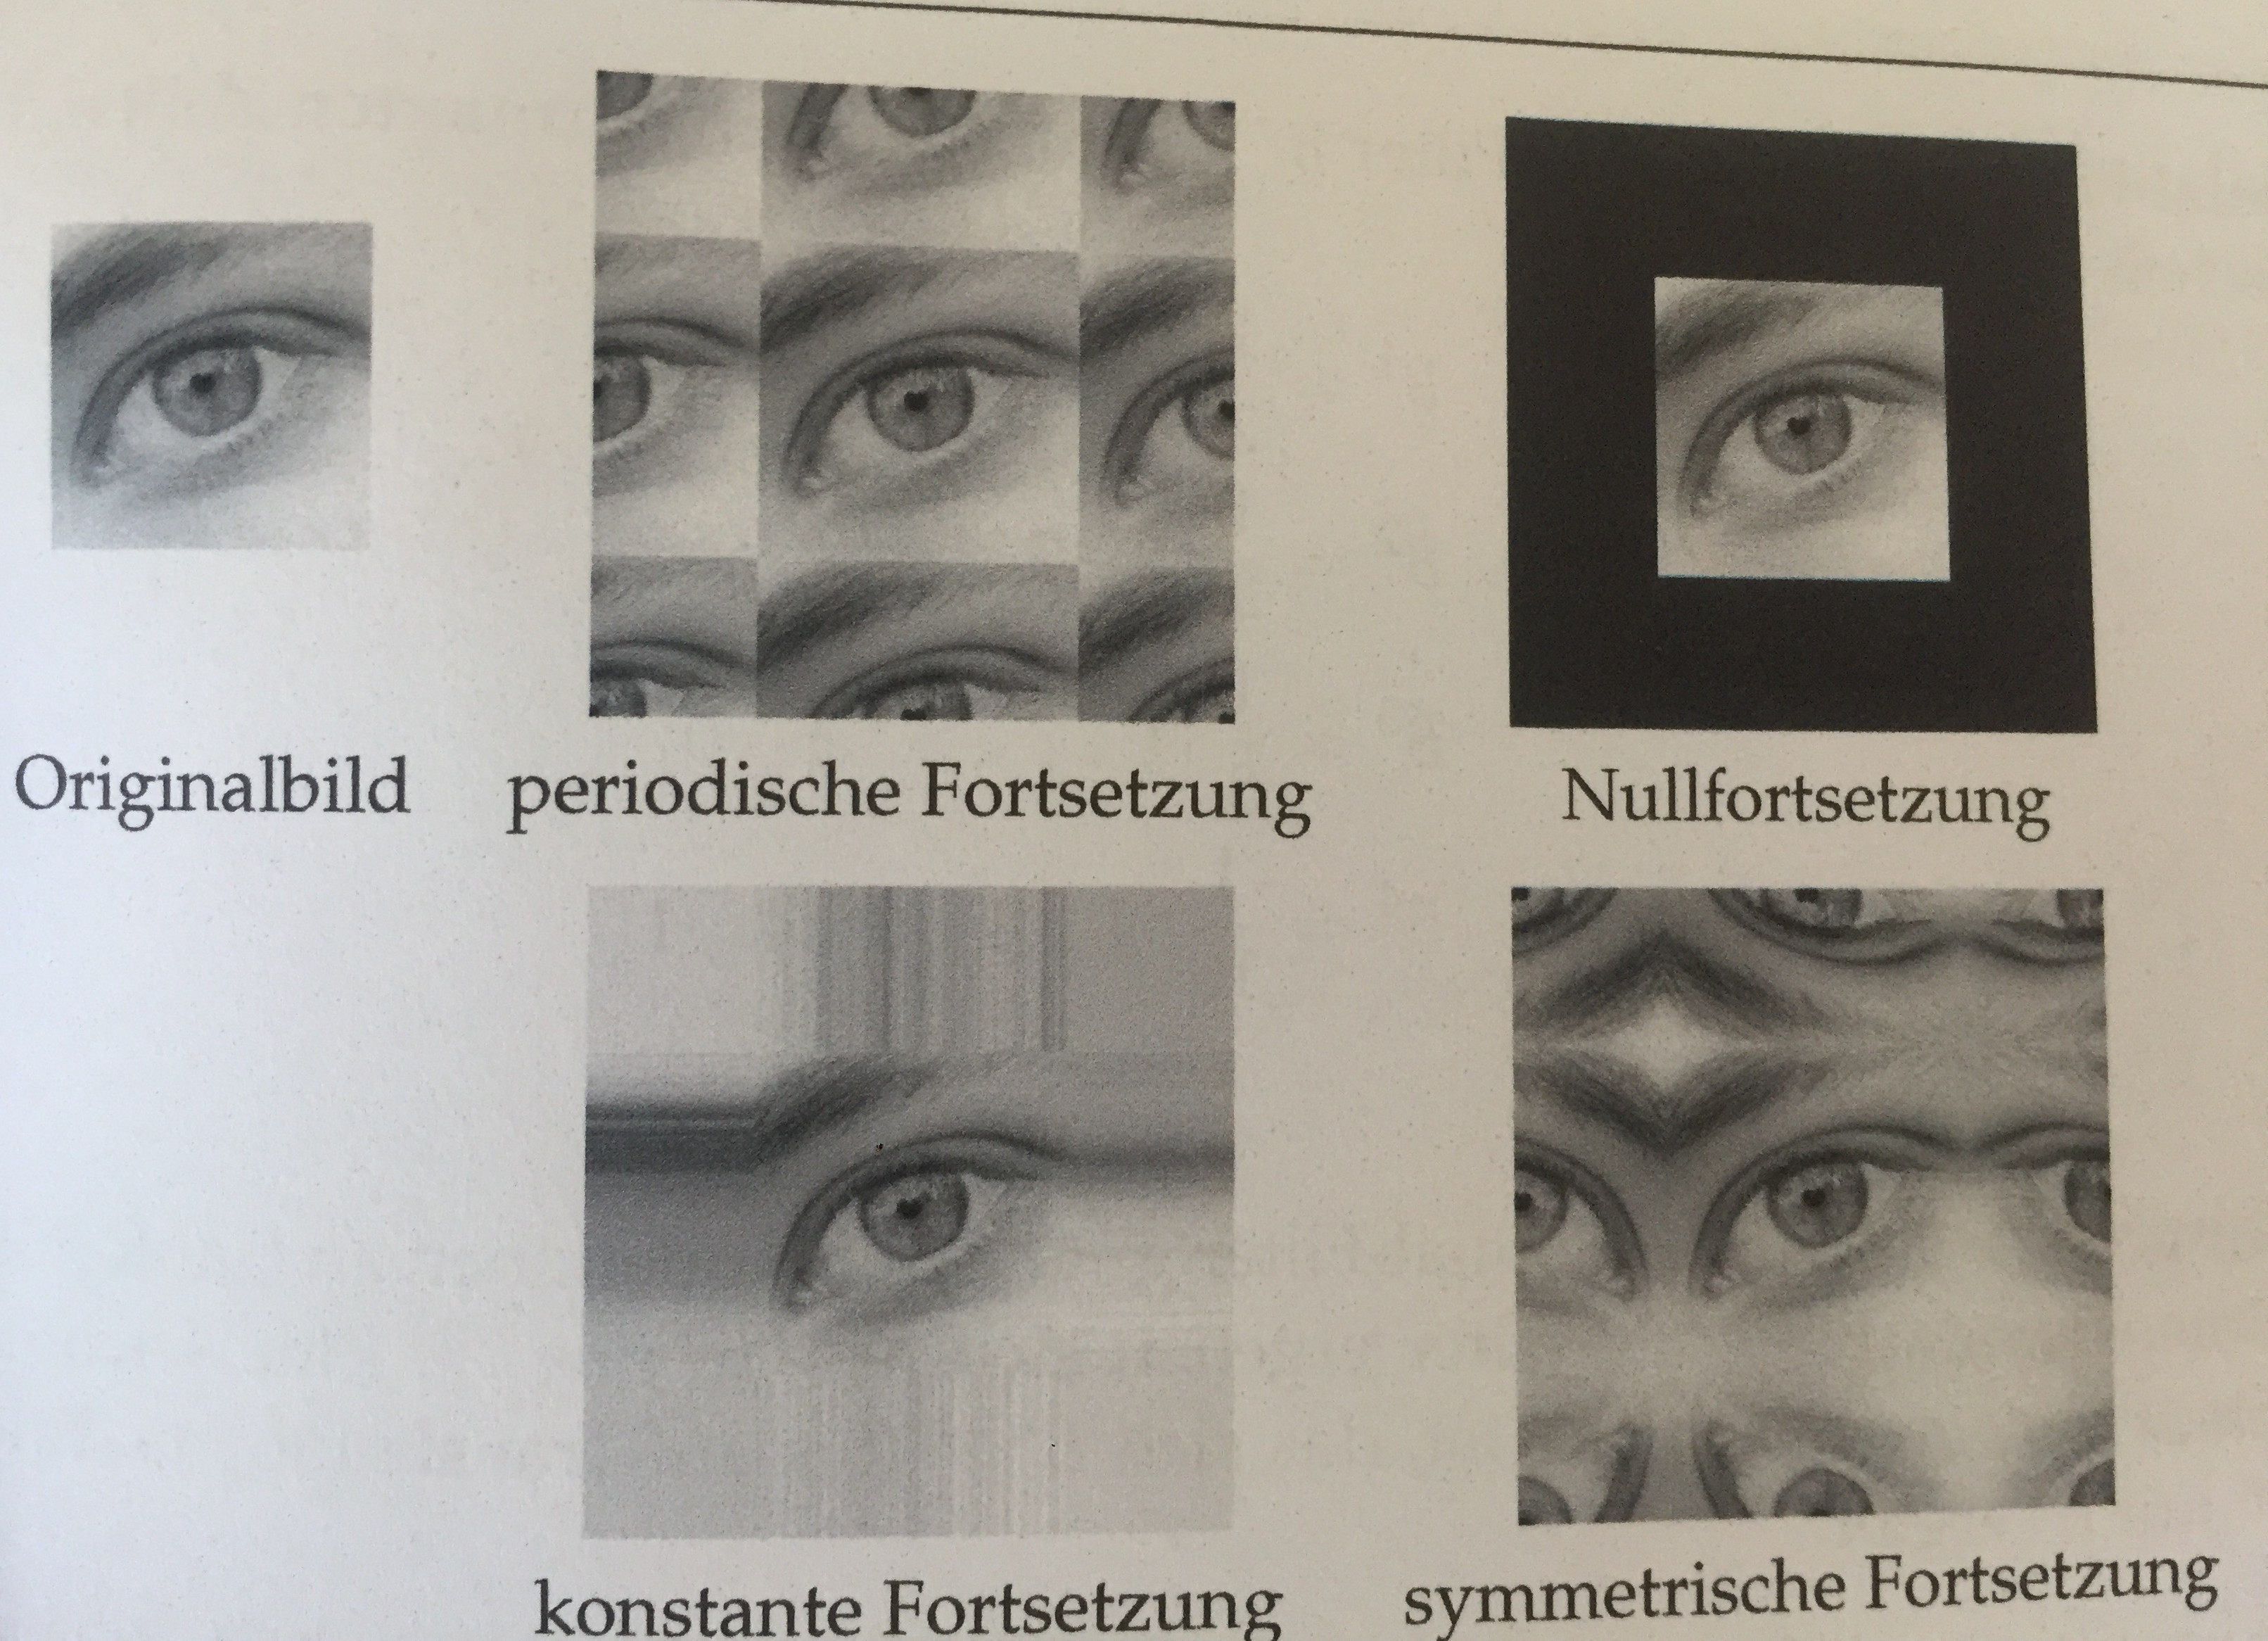
\includegraphics[width=0.7\textwidth]{img/tile}
      \caption{Quelle: Mathematische Bildverarbeitung; Breies, Lorenz}
\end{figure}
\end{block}
 \end{frame}


\begin{frame}
    \frametitle{Lineare Filter}
\framesubtitle{}
\begin{block}{Fortsetzung am Bildrand}
\begin{align*}
& \text{Periodische Fortsetzung } \tilde{U}_i = U_{i \text{ mod } N} \\
& \text{Nullfortsetzung } \tilde{U}_i = U_{i} \text{ für } 0 \leq i \leq N; \; 0 \text{ sonst} \\
& \text{Konstante Fortsetzung } \tilde{U}_i = U_{P_N(i)}; \; P_N(i) = max(min (N-1,i ), 0) \\
& \text{Symmetrische Fortsetzung (spiegeln + periodisch) } \\
& \tilde{U}_i = U_{Z_N(i \text{ mod } 2 N)}; \; Z_N(i) = min (i, 2N-1-i ) \\
\end{align*}

\end{block}
 \end{frame}

\begin{frame}
    \frametitle{Lineare Filter}
\framesubtitle{}

\begin{block}{Schachtelung von Filtermasken}
\begin{align*}
(U * H) * G =  U * (H \cdot G)
\end{align*}

\end{block}

 \end{frame}


\begin{frame}
    \frametitle{Lineare Filter}
\framesubtitle{}

\begin{block}{Gleitendes Mittel}
Das gleitende Mittel ist definiert durch 
\begin{align*}
(M^n)^t \cdot M^n 
\end{align*}
mit $M^n = \frac{1}{n}  \begin{bmatrix}  1 & \ldots 1\end{bmatrix}$.
\end{block}

 \end{frame}


\begin{frame}
    \frametitle{Lineare Filter}
\framesubtitle{}

\begin{block}{Gauß-Filter}
Der Gauß-Filter $G^\sigma$ mit Varianz $\sigma >0$ ist definiert durch  
\begin{align*}
\hat{G^\sigma}_{k,l} = \exp \biggl( \frac{-(k^2 + l^2)}{2 \sigma^2} \biggr), \; G^{\sigma} = \frac{\hat{G^\sigma}}{\sum_{k,l} \hat{G^\sigma}_{k,l}}
\end{align*}

\end{block}

 \end{frame}



\begin{frame}
    \frametitle{Lineare Filter}
\framesubtitle{}

\begin{block}{Binomial-Filter}
Der Binomial-Filter $B^n$ ist definiert durch $(B^n)^t \cdot B^n$ mit $B^n := \frac{1}{2^{n}} P(n)$, wobei $P(n)$ die n-te Reihe des Pascalschen Dreiecks ist. 
\begin{align*}
B^1 :=  \frac{1}{2} \begin{bmatrix}  1 & 1 \end{bmatrix} \\
B^2 :=  \frac{1}{4} \begin{bmatrix}  1 & 2 & 1\end{bmatrix} \\
B^3 :=  \frac{1}{8} \begin{bmatrix}  1 & 3 & 3 & 1\end{bmatrix} \\
B^4 :=  \frac{1}{16} \begin{bmatrix}  1 & 4 & 6 & 4 & 1\end{bmatrix} \\
\vdots
\end{align*}

\end{block}

 \end{frame}



\begin{frame}
    \frametitle{Lineare Filter}
\framesubtitle{}

\begin{block}{Differenzenquoienten}
Wir approximieren eine eindimensionale Ableitung durch  Differenzenquotient 
\begin{align*}
(\text{Vorwärts}) \; f'(x) \approx \frac{f(x +h )- f(x) }{h} \\
(\text{Rückwärts}) \; f'(x) \approx \frac{f(x)- f(x -h) }{h} \\
(\text{Zentral}) \; f'(x) \approx \frac{f(x +h)- f(x -h) }{2h} 
\end{align*}
 
\end{block}
 \end{frame}

\begin{frame}
    \frametitle{Lineare Filter}
\framesubtitle{}

\begin{block}{Partielle Ableitungen}
\begin{align*}
& D_x^+:= \begin{bmatrix}  0 & -1 & 1\end{bmatrix} ; \; D_x^-:= \begin{bmatrix}  -1 & 1 & 0\end{bmatrix} ;\: D_x:= \begin{bmatrix}  -1 & 0 & 1\end{bmatrix} \\
& D_y^+ :=  \begin{bmatrix}  0 \\ -1 \\ 1\end{bmatrix} ; \; D_y^- :=  \begin{bmatrix}  -1 \\ 1 \\ 0\end{bmatrix} ; \; D_y :=  \begin{bmatrix}  -1 \\ 0 \\ 1\end{bmatrix} 
\end{align*}

\end{block}
 \end{frame}



\begin{frame}
    \frametitle{Lineare Filter}
\framesubtitle{}

\begin{block}{Prewitt Filter}
Der Prewitt Filter ist die Kombination einer partiellen Ableitung mit einer Mittelung
\begin{align*}
P_x  = \frac{1}{3}\begin{bmatrix}  1 \\ 1 \\ 1\end{bmatrix} \cdot  \begin{bmatrix}  -1 & 0 & 1\end{bmatrix} =  \frac{1}{6} \begin{bmatrix}  -1 & 0 & 1 \\ -1 & 0 & 1 \\ -1 & 0 & 1 \end{bmatrix} \\
P_y  = \begin{bmatrix}  -1 \\ 0 \\ 1\end{bmatrix} \cdot   \frac{1}{3} \begin{bmatrix}  1 & 1 & 1\end{bmatrix} = \begin{bmatrix}  -1 & -1 & -1 \\ 0 & 0 & 0 \\ 1 & 1 & 1 \end{bmatrix} 
\end{align*}

\end{block}
 \end{frame}

\begin{frame}
    \frametitle{Lineare Filter}
\framesubtitle{}

\begin{block}{Sobel Filter}
Der Sobel Filter ist die Kombination einer partiellen Ableitung mit einem Gauß-Filter
\begin{align*}
S_x  = \begin{bmatrix}  1 \\ 2 \\ 1\end{bmatrix} \cdot  \begin{bmatrix}  -1 & 0 & 1\end{bmatrix} = \begin{bmatrix}  -1 & 0 & 1 \\ -2 & 0 & 2 \\ -1 & 0 & 1 \end{bmatrix} \\
S_y  = \begin{bmatrix}  -1 \\ 0 \\ 1\end{bmatrix} \cdot  \begin{bmatrix}  1 & 2 & 1\end{bmatrix} = \begin{bmatrix}  -1 & -2 & -1 \\ 0 & 0 & 0 \\ 1 & 2 & 1 \end{bmatrix} 
\end{align*}

\end{block}
 \end{frame}


\begin{frame}
    \frametitle{Lineare Filter}
\framesubtitle{}

\begin{block}{Laplace Filter}
Die zweite Ableitung lässt sich mit einem Vorwärts- und einem Rückwärts-Differenzenquotient  approximieren und man erhält damit $D_{x^2} =  \begin{bmatrix}  1 & -2 & 1\end{bmatrix} $ und 
 $D_{y^2} =  \begin{bmatrix}  1 \\ -2 \\ 1\end{bmatrix}$. Der Laplace Filter ist analog zum Laplace-Operator definiert durch 
\begin{align*}
\triangle  = D_{x^2}  + D_{y^2}  = \begin{bmatrix}  1 \\ -2 \\ 1\end{bmatrix}  +  \begin{bmatrix}  1 & -2 & 1\end{bmatrix} = \begin{bmatrix}  0 & 1 & 0 \\ 1 & -4 & 1 \\  0 & 1 & 0 \end{bmatrix} 
\end{align*}

\end{block}
 \end{frame}




\end{document}
